\documentclass[12pt]{article}

\usepackage{graphicx}
\usepackage{amsmath}
\usepackage{amssymb}

\usepackage{color}
\usepackage[total={6in,8in}]{geometry}
\usepackage{amsthm}

\usepackage{enumitem}
\usepackage{centernot}

\newcommand{\N}{\mathbb{N}}
\newcommand{\Z}{\mathbb{Z}}
\newcommand{\Q}{\mathbb{Q}}
\newcommand{\R}{\mathbb{R}}
\newcommand{\C}{\mathbb{C}}
\newcommand{\sn}{\mathfrak{S}}
\newcommand{\ve}{\varepsilon}
\setlength{\parindent}{1cm}


\author{Marika Swanberg}

\begin{document}
Marika Swanberg. Collaborators: Jillian James, \today
\bigskip 

\begin{enumerate}
\item 
\begin{enumerate}
\item I decided that I wanted to keep the runtime more or less constant, so I used the following formula for Python:
\begin{equation*}
SIZE = 2^i, \text{ and }
ITERS = 2^{(25-i)}
\end{equation*}
\item I reran some of the points that were outliers, and chose the number that I got when I reran it because the rerun always ended up looking less like an outlier. (not very scientific though).
\item See Figure 1 on the next page for Python data (I couldn't get the figures formatted correctly so I just put them on a separate page)
\end{enumerate}
\item I changed my formula a little, because the C code was much much faster than the Python. I increased the number of iterations by $2^5$-fold:
\begin{equation*}
SIZE = 2^i, \text{ and }
ITERS = 2^{(30-i)}
\end{equation*}
\item After porting this to C and running it on different types, I found a few distinct patterns (see Figure 2 on page 3) The first thing that I noticed is the sharp increase in time per memory access after a given object size for each different datatype ($2^{12}$ for int64 and double, $2^{14}$ for int16, int32, and float, and $2^{15}$ for int8, roughly). I concluded that this must be due to one of the memory caches filling up. 

Another interesting trend is the way that these datatypes are grouped. I assume this is because of the amount of memory that each type takes up.

In addition, if you squint at the graph, you can almost see three levels, which I think may represent the 3 caches (but I could be wrong).

\item In order to determine the amount of memory used for each of the different C datatypes with $2^{20}$ objects, we use the command /usr/bin/time -v ./update 1048576 1, and then read the "maximum resident set size (kbytes)" result.

\begin{center}
\begin{tabular} {| c | c |} 
\hline
datatype & memory usage (kb) \\
\hline
int64\_t & 50164 \\
double & 50128 \\
\hline
float & 25606 \\
int32\_t & 25600 \\
\hline
int16\_t & 13184 \\
\hline
int8\_t & 7140 \\
\hline
\end{tabular}
\end{center}

\pagebreak
\end{enumerate}

\begin{figure}
\centering
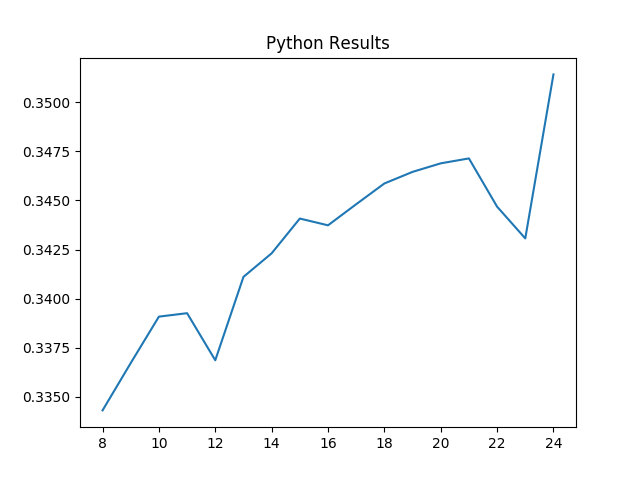
\includegraphics[width=\linewidth]{Python_Results.png}
\caption{This is what Python looks like. It is slow}
\end{figure}

\begin{figure}
\centering
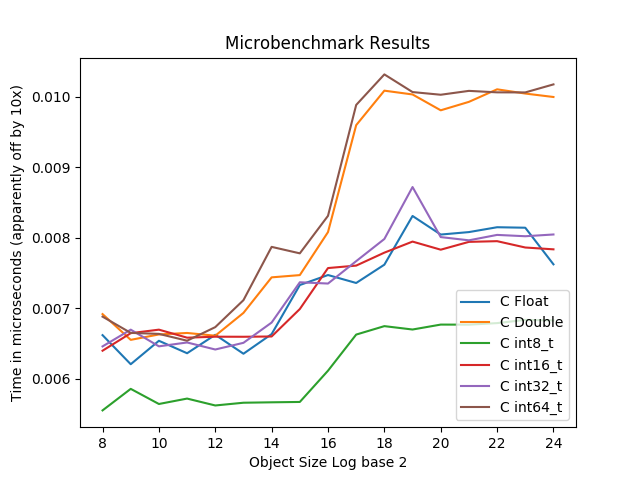
\includegraphics[width=\linewidth]{All_C_Results.png}
\caption{Look at the memory caches filling up. I wrote this on the y-axis label, but I will reiterate that apparently, according to people who know things about computer systems (Eitan and my mother) my measurements are 10x too fast to be feasible. I could not manage to find the bug in my calculations. I timed these with a stopwatch to see if I was going crazy and my timing calculations in the C code do not seem off by 10, according to the stopwatch.}
\end{figure}

\begin{figure}
\centering
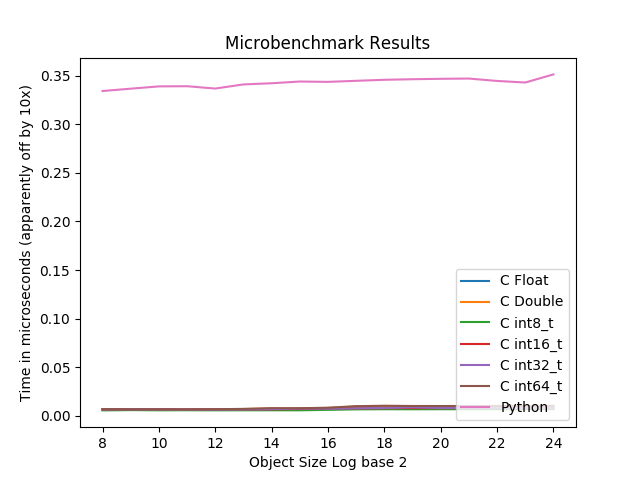
\includegraphics[width=\linewidth]{All_Results.png}
\caption{Look how slow Python is.}
\end{figure}
\end{document}